\documentclass[11pt,letterpaper]{article}
\usepackage[margin=2.5cm,top=3.5cm,bottom=3cm]{geometry}
\usepackage{booktabs}
\usepackage{graphicx}
\usepackage[hidelinks]{hyperref}
\usepackage{microtype}
\usepackage[table,dvipsnames]{xcolor}
\usepackage{longtable}
\usepackage{array}
\usepackage{caption}
\usepackage[T1]{fontenc}
\usepackage{lmodern}
\usepackage{fancyhdr}
\usepackage{amsmath}
\usepackage{titlesec}
\usepackage{enumitem}

\definecolor{wavblue}{RGB}{26,58,92}
\definecolor{wavgray}{RGB}{120,120,120}
\definecolor{wavlight}{RGB}{235,242,250}
\definecolor{wincolor}{RGB}{0,110,0}

\graphicspath{{/Users/egs/repos/waverider/benchmarks/canonical_tests/}}

\pagestyle{fancy}
\fancyhf{}
\fancyhead[L]{\small\color{wavgray}Manifold-Informed Architecture Benchmark \textemdash\ IRIS}
\fancyhead[R]{\small\color{wavgray}\texttt{waverider @ 4b8002e}}
\fancyfoot[C]{\small\color{wavgray}\thepage}
\renewcommand{\headrulewidth}{0.4pt}

\titleformat{\section}{\large\bfseries\color{wavblue}}{}{0em}{}[\color{wavblue}\titlerule]
\titleformat{\subsection}{\normalsize\bfseries\color{wavblue}}{}{0em}{}
\setlength{\parindent}{0pt}
\setlength{\parskip}{4pt plus 1pt}

\begin{document}

\begin{center}
  {\LARGE\bfseries\color{wavblue} Manifold-Informed Architecture Benchmark}\\[6pt]
  {\large IRIS: 3 classes, 4D input}\\[8pt]
  {\small Generated: 2026-04-14 20:54:32 \quad$|$\quad Apple M5 Max MacBook Pro, 64 GB RAM, 2TB SSD}\\[2pt]
  {\small\texttt{waverider @ 4b8002e} (--abbrev-re
4b8002ee9a2e3d56a219d7dab695a80b8efd1e07) \quad$|$\quad 2026-04-14 20:51:52 -0400}
\end{center}
{\color{wavblue}\noindent\rule{\linewidth}{1.5pt}}
\medskip

\noindent\colorbox{wavlight}{\parbox{\dimexpr\linewidth-2\fboxsep\relax}{
  \smallskip
  \textbf{Best:} Standard (16$\rightarrow$8)\quad test acc $= 0.9444 \pm 0.0157$\\[2pt]
  \textbf{Manifold:} 4D $\rightarrow$ 3D (25.0\%\ noise dimensions)\\[2pt]
  \smallskip
}}
\bigskip

\section{Experimental Setup}

\begin{tabular}{@{}ll@{}}
\toprule
\textbf{Parameter} & \textbf{Value} \\
\midrule
  Dataset & IRIS \\
  Input dimensionality & 4D \\
  Classes & 3 \\
  Intrinsic dim ($d$) & 3 \\
  Variance threshold ($\tau$) & 0.9 \\
  Epochs & 150 \\
  Trials & 3 \\
\bottomrule
\end{tabular}

\section{Manifold Discovery}

Local PCA over the training set, $k = ?$ neighbors. Intrinsic dimensionality $d$ is taken as the maximum per-class maximum at $\tau = 0.9$, clamped to $n_{\mathrm{classes}} = 3$.

\begin{tabular}{@{}rrrrrr@{}}
\toprule
$\tau$ & Mean $d$ & Std & Min & Max & Noise (\%) \\
\midrule
  0.95 & 3.2 & 0.5 & 2 & 4 & 19.0 \\
  0.90 & 2.8 & 0.4 & 2 & 4 & 29.6 \\
  0.85 & 2.5 & 0.5 & 1 & 3 & 38.3 \\
  0.80 & 2.1 & 0.4 & 1 & 3 & 46.2 \\
\bottomrule
\end{tabular}

\subsection{Per-Class Intrinsic Dimensionality}

\begin{tabular}{@{}lrrrr@{}}
\toprule
Class & Mean $d$ & Std & Min & Max \\
\midrule
  virginica & 2.8 & 0.4 & 2 & 3 \\
  setosa & 2.7 & 0.5 & 2 & 3 \\
  versicolor & 2.7 & 0.5 & 2 & 3 \\
\bottomrule
\end{tabular}

\section{Architecture Comparison}

{\small
\begin{tabular}{@{}p{7cm}rccr@{}}
\toprule
\textbf{Architecture} & \textbf{Params} & \textbf{Test Acc ($\mu \pm \sigma$)} & \textbf{Loss} & \textbf{Acc/Kparam} \\
\midrule
  {\color{wincolor}Standard (16$\rightarrow$8)\,$\star$} & 243 & $0.9444 \pm 0.0157$ & 0.1574 & 3.8866 \\
  {Wide Manifold (4d$\rightarrow$2d$\rightarrow$d, d=3)} & 171 & $0.9444 \pm 0.0157$ & 0.1817 & 5.5231 \\
  {Manifold (2d$\rightarrow$d, d=3)} & 63 & $0.8778 \pm 0.0314$ & 0.3069 & 13.9330 \\
  {PCA$\rightarrow$3D + MLP (2d$\rightarrow$d)} & 57 & $0.9000 \pm 0.0272$ & 0.2405 & 15.7895 \\
  {Intrinsic Dim (PCA$\rightarrow$3D$\rightarrow$output)} & 24 & $0.7889 \pm 0.0416$ & 0.4703 & 32.8704 \\
\bottomrule
\end{tabular}
}

\smallskip
{\small $\star$ = best performing architecture}

\section{Key Findings}

\begin{itemize}[leftmargin=*,itemsep=3pt]
  \item \textbf{Best architecture:} Standard (16$\rightarrow$8) \textemdash\ test accuracy $0.9444 \pm 0.0157$
  \item \textbf{Manifold compression:} 4D $\rightarrow$ 3D (25.0\%\ of ambient dimensions carry no structure)
\end{itemize}

\clearpage
\section{Result Figure}

\begin{figure}[htbp]
\centering
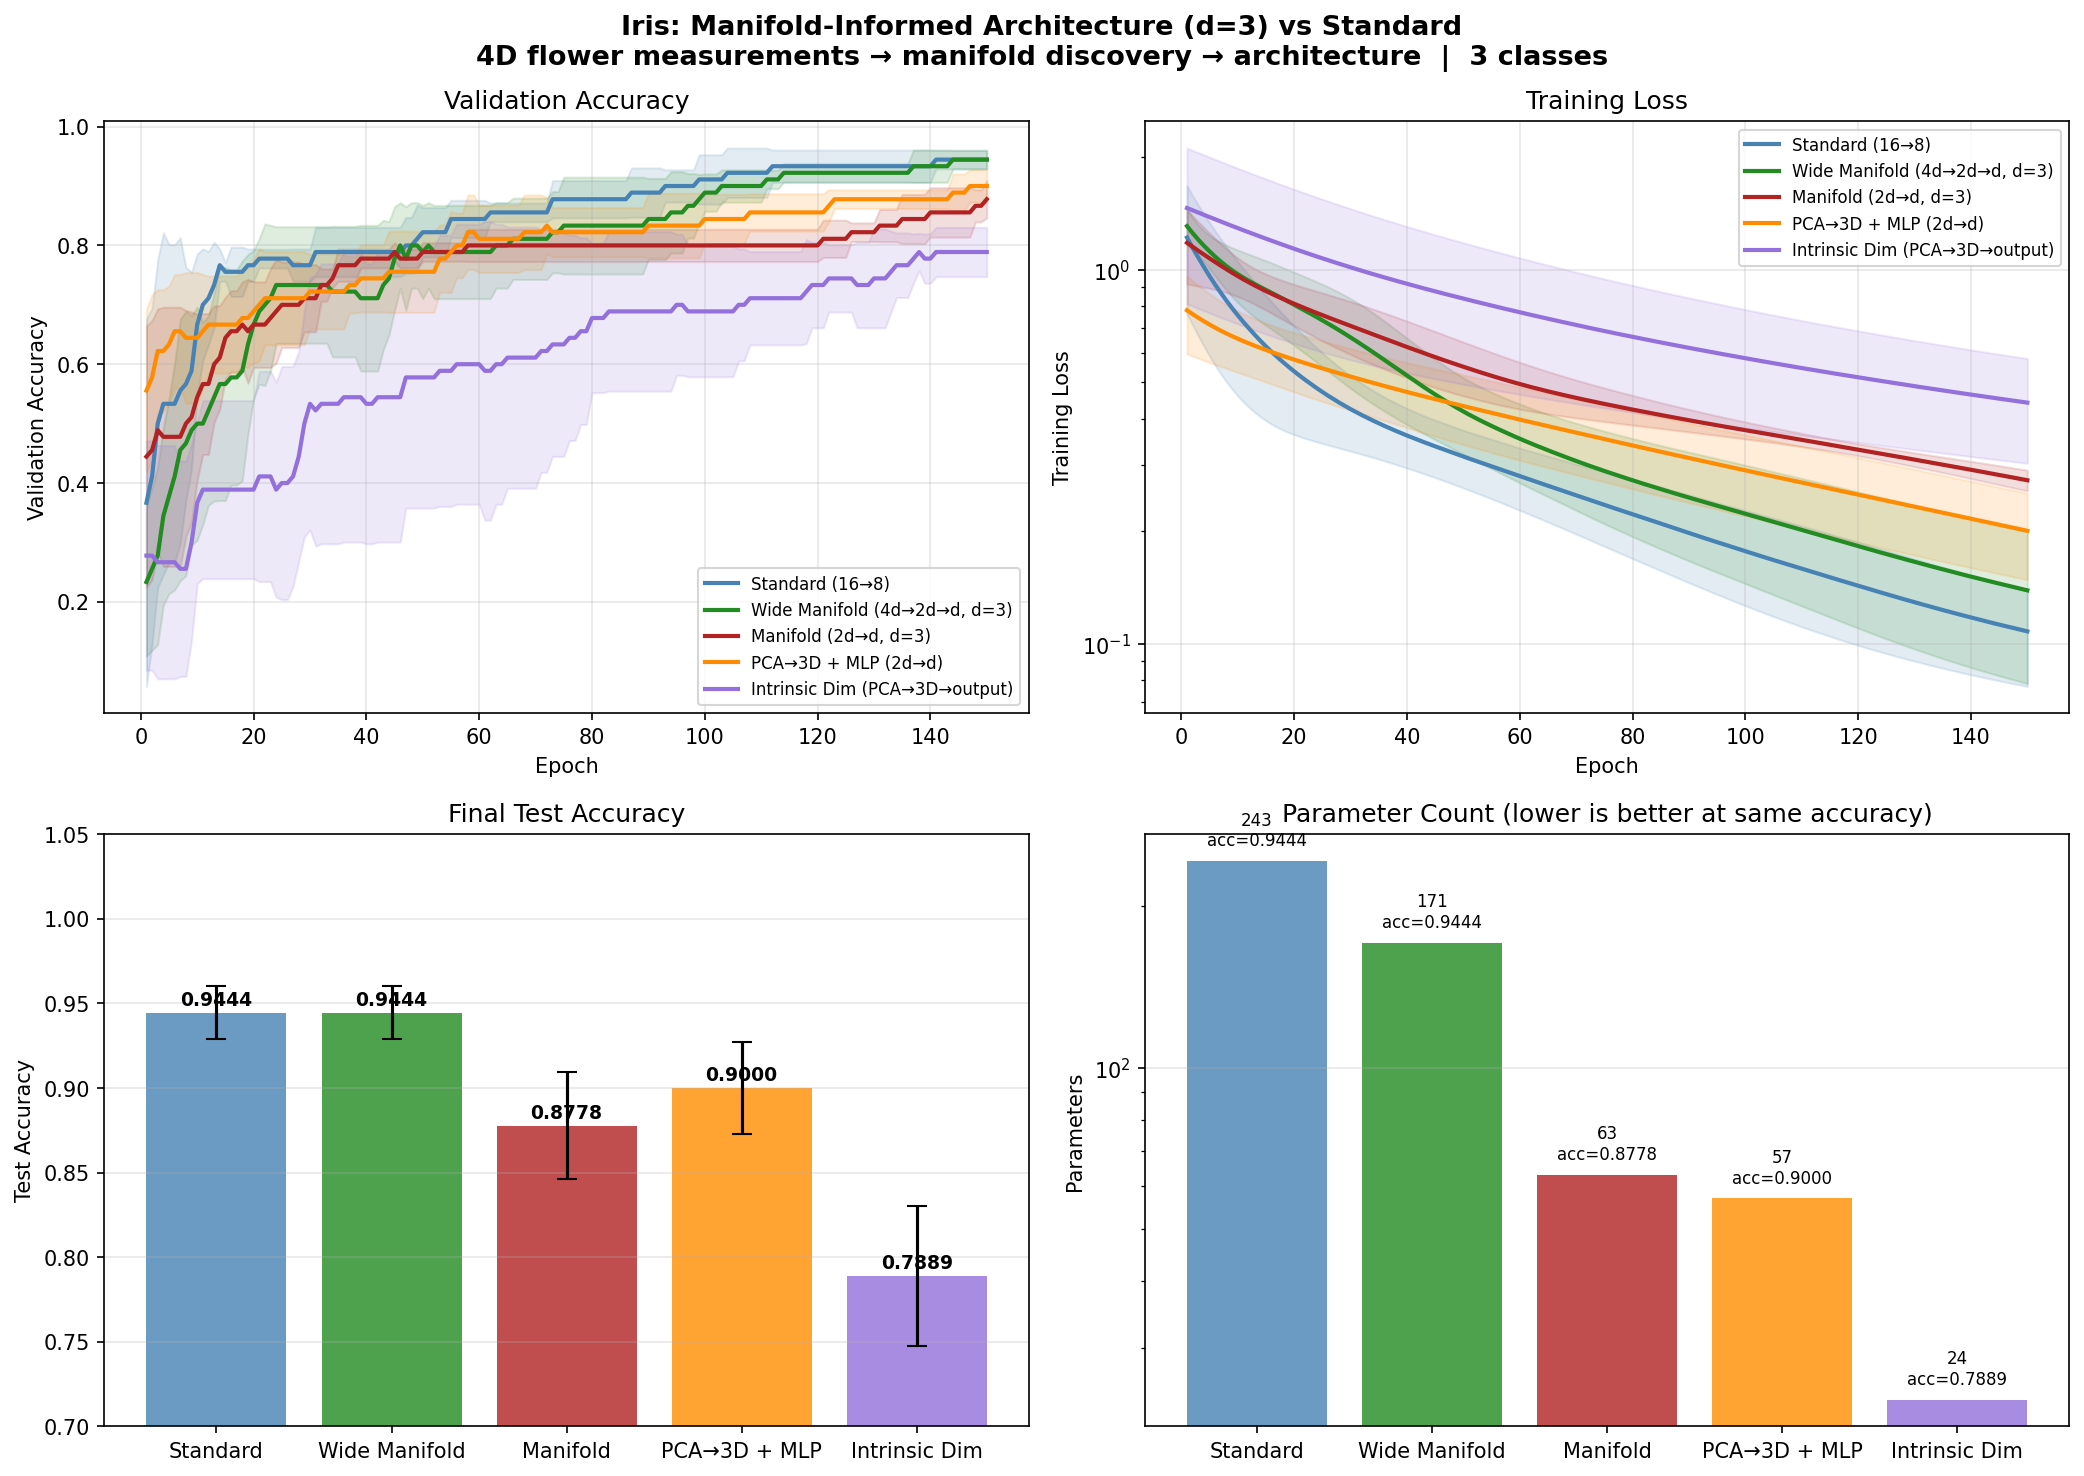
\includegraphics[width=\textwidth]{iris_architecture_results}
\caption{IRIS manifold-informed vs.\ standard architecture comparison. $d = 3$, 150 epochs, 3 trials.}
\end{figure}

\section{Provenance}

\begin{tabular}{@{}ll@{}}
\toprule
\textbf{Item} & \textbf{Value} \\
\midrule
  Repository & \href{https://github.com/Flux-Frontiers/waverider}{Flux-Frontiers/waverider} \\
  Commit & \texttt{4b8002e} (--abbrev-re
4b8002ee9a2e3d56a219d7dab695a80b8efd1e07) \\
  Commit date & 2026-04-14 20:51:52 -0400 \\
  Commit message & add: cifar10 results \\
  Python & 3.12.13 \\
  TensorFlow & 2.16.2 \\
  Device & CPU (forced) \\
  Host & Turing \\
  OS & macOS-26.4-arm64-arm-64bit \\
  Machine & Apple M5 Max MacBook Pro, 64 GB RAM, 2TB SSD \\
  Generated & 2026-04-14 20:54:32 \\
\bottomrule
\end{tabular}

\end{document}
